\chapter{Introduction}
\section{General aspects}
The technological evolution in the field of micro aircraft brings multiple benefits in many field of applications. Many industrial sectors benefits from the use of these devices, some examples are agricultural engineering, package delivery, but also security and military industry. The main interest concerns especially drones that have four rotors, also called quadcopters. The rapid expansion of the drone industry for civil contexts has overwhelmed the regulations in the use of them in terms of safety and control. While in the military context the development of surveillance system keeps up with the evolution of drones, the same is not true for civilian surveillance and defense. Consequently, these tools can be used to carry out illegal actions and crimes without being easily thwarted with civil technologies but only with sophisticate and expensive systems. Is important to consider that in recent times the drone's technology has undergone an incredible development mainly in the civil field. In fact, the recent diffusion of drones for commercial use has undergone an exponential growth. \\ Mosts significant causes for the drones's success is the ease of use and the low cost. In fact, anyone nowadays can easily get and use a drone even without having any experience in this field. On the other hand, due to the incredible spread of drone, the first regulations are being born in this period such as the driving license, or the drone no fly zones \cite{survey}. These regulations are really difficult to verify and control in a simple way. The security aspect acquires greater importance as these devices are easily accessible and easy to use by anyone. In this way the drones are able to carry out many illegal actions in a simple way and allow ill-intentioned users to escape the controls of the police. So the drones are also a good instruments to carry out terrorism and illegal operations like transporting illegal objects, weapons, bombs, etc.\\ How it is possible to to contrast illegal action and put into practice the drones's regulations easily?\\
Considering the current development of commercial drones such as their velocity, their range and their battery duration, is very difficult to protect an area against unauthorized flying drone by using non military equipments. This denotes that there isn't an equal technological level for the side of civilian defence devices, so the imbalance between commercial drone and civilian defense technology is very great. So the infringements of the rules became difficult to detect and contrast. While in the military context drones have been used for several years and the technologies of contrast and protection are very advanced. Then obviously it is not possible to use military solutions in the civilian context, for a matter of high costs but above all for the security of the close people. While there is a large increase in documented and verified accidents due to civilian drones, as we can understand, on the other hand there is no simple civilian security system for drone defense. For example in the military technologies one of the less invasive techniques of drone neutralization is the jamming, that do not involve the use of physical weapons and the main objective is to interfere with the flight of the drone. Despite the absence of physical weapons in a civilian context, it cannot be used due to the interference caused to other communications. For example the existing wireless network system or wireless sensors network would be temporarily paralyzed. \\ The impossibility to use a jamming approach in presence of people is also due to the possible fall down of the drone, that in relation to it's velocity and it's mass can cause serious problems and incidents, also if we consider that it can transport explosive. \\ The detection solutions for drone defense are many and of different nature, each with its own pros and cons \cite{survey} \cite{uspace} \cite{robinradar1}. There is no single and complete solution, in fact, the use of several systems at the same time called hybrid systems is preferred. \\ The main attention of this thesis is put on the first phase of drone defense in civil context that is the detection phase and the technology investigated is the radar one. Several type of radars are used today to contrast drone also in civilian context but the cost of these devices is very high. The principal aim is to detect and to understand if there is a possible threat in the supervised area by means of a cost accessible radar technology. It's important to consider that the detection capability includes also the ability to identify an unauthorized drone. This means that detection instruments must be able to distinguish between drone and other flying object as birds, and then it must be capable to understand if the drone is legal or illegal, for example by analyzing it's flying path. Usually the contexts area in a civil environment is a crowded events such as concert or a sport event, where the large number of people makes security checks very difficult and exposes the context to a high terrorist attack risk. In these cases, the vulnerability to illegal drones used to carry explosives is very high. This is one of the most critical cases, but drone defense can be very useful even in less critical cases. For example, it could be very useful to block a drone carrying a symbol of violence capable of causing clashes and unrest, as happened several times during international sporting events characterized by political tensions. Another field of application of less critical case is the protection of privacy and confidentiality that doesn't cause serious risk to people safe but is at the same time important. For example an unauthorized drone can be used to spy a confidential site like industrial production site.\\ More close to individual context, can be the protection of individual houses or boat where people may have a significant need to protect their privacy. Another field of application could be the prisons, where drones could be used to transport objects from the outside. All these context are characterized by the need of low cost, portable and ease of use detection instruments that is not possible to find in the military solutions.\\ Some of the drone detection solutions used today are based on optical/thermal vision, radar, acoustic and radio frequencies technologies but these are characterized by high costs and complexity. The focus is put on the radar technologies and the aim is to find an optimal solution for all these cited civil context characterized by the presence of people near to the detection radar. The idea is to achieve low cost and low complexity solutions that permit to put radar technologies for drone defense in the market for civilian people considering that the possibility to use military system is eliminated.

\begin{figure}[h!]
    \centering
    \includegraphics[width=12cm]{imgs/Drone delivery.jpg}
    \caption{Quadcopter drone in package delivery.}
\end{figure}




\section{Motivations}
The motivations that drive the research and development of drone defense can be deduced from the documented cases of accidents and attacks on public safety that have been made by means of drones \cite{survey} \cite{uspace}. It is important to note that the drones we are talking about are not those used in war, but the simple commercial drones that can be purchased in any electronics store. There are many and different cases in which the defense against unauthorized drones is of significant importance. For simplicity we can divide the application cases into two large groups: military cases and civil cases. This is why it is important to evaluate the level of risk and the context in order to choose the appropriate defense technologies. Faced with a very high risk in a very large area such as in an airport, it is necessary to use a military-grade technology that therefore requires high costs and high complexity. Faced with a less extensive risk that concerns an area of limited size, as in the case of a public event, a civil defense technology becomes necessary and therefore it requires low cost but at the same time portability and ease to deploy/use. Several documented events highlight the need for a good defense against unauthorized use of drones are shown below \cite{survey}.
As for the military field, documented cases in airports show how traffic can be blocked by the presence of unauthorized drones near airport runway. For example in December 2018 at Gatwick Airport, the second largest airport in England, air traffic was blocked for a day due to the presence of unauthorized drone flying over the runaway. The instrument used for ATC (Air Traffic Control) in 2018 were unable to detect a very small object close to the instruments. The same thing happened at the Frankfurt Airport in Germany in May 2019 \cite{survey}. The drones managed to reach crucial areas for air traffic without being detected by the existing radar systems due to their small RCS and close proximity to the devices. Other dangerous events attributed to military-grade cases are attacks on public institutions. One of the most recent cases documented is the attack on Saudi Arabia's largest oil refinery in September 2019, using 10 explosives-carrying drones \cite{survey}. Obviously in this case of attack the drones were more sophisticated than simple commercial ones and were of military level. So it's preferable to use also a military grade level defense system in this cases because in a context like an airport or an oil refinery is possible to use expensive devices and complex solution to guarantee the security. \\ Let's now focus on the most significant cases for the purpose of the thesis, those concerning individual objectives or public events where it is not possible to use military-level equipment. A first documented case is the attack on the home of the Japanese prime minister in April 2015 \cite{survey}, where for obvious reasons it is not possible to install military protective equipment. Precisely in these conditions, the need for a portable, simple and low-cost detection system becomes very clear. Some examples of military-grade attacks carried out using commercial-grade drones are provided by the old Islamic State (IS). The first documented case that discloses the possibility of using common commercial drones to carry out attacks occurred in Syria in October 2016, when the IS murdered two Iranians using drones bought on Amazon \cite{survey}. This event makes the concept of how simple it is to carry out illegal actions by means of commercial drones very clear. There was also the first case of attempted assassination of a head of state by means of drone, that it's what happened to Venezuelan president Nicolas Maduro in August 2018 \cite{survey}. During a public event, two common commercial drones carrying bombs tried to hit it, fortunately it did not go well. For what concern the public events, one of the most famous case of non authorized drone was in October 2014 during the national football match Serbia-Albania: a drone invaded the playing field carrying a political-military symbol that caused serious clashes and unrest preventing the continuation of the game. \\ Given the enormous availability and the ever lower cost of commercial drones, the urgent need for detection devices of the same level is very clear. The same level means the ease of use, low cost and portability of detection systems. Considering that commercial drones can achieve velocities that goes from several km/h up to 140 km/h. %It's a problem also the too low velocity because it's necessary a radar with a very high resolution in frequency to detect them.
The maximum range achievable by a commercial controlled drone can vary from 2-3 km up to 10 km so the range is also an important parameter to design a radar instrument. Also the range in altitude, of about 6 km, is a critical parameter. Considering the small dimensions of a drone at this altitude is impossible to see it with naked eye. Especially in conditions of temporary events a quick installation becomes possible thanks to the ease of deployment and portability of instruments. Furthermore, the ease of transport and use combined with less expensive radar technology can fully satisfy the need in civil and crowded contexts described in the next section. 

\begin{figure}[h!]
    \centering
    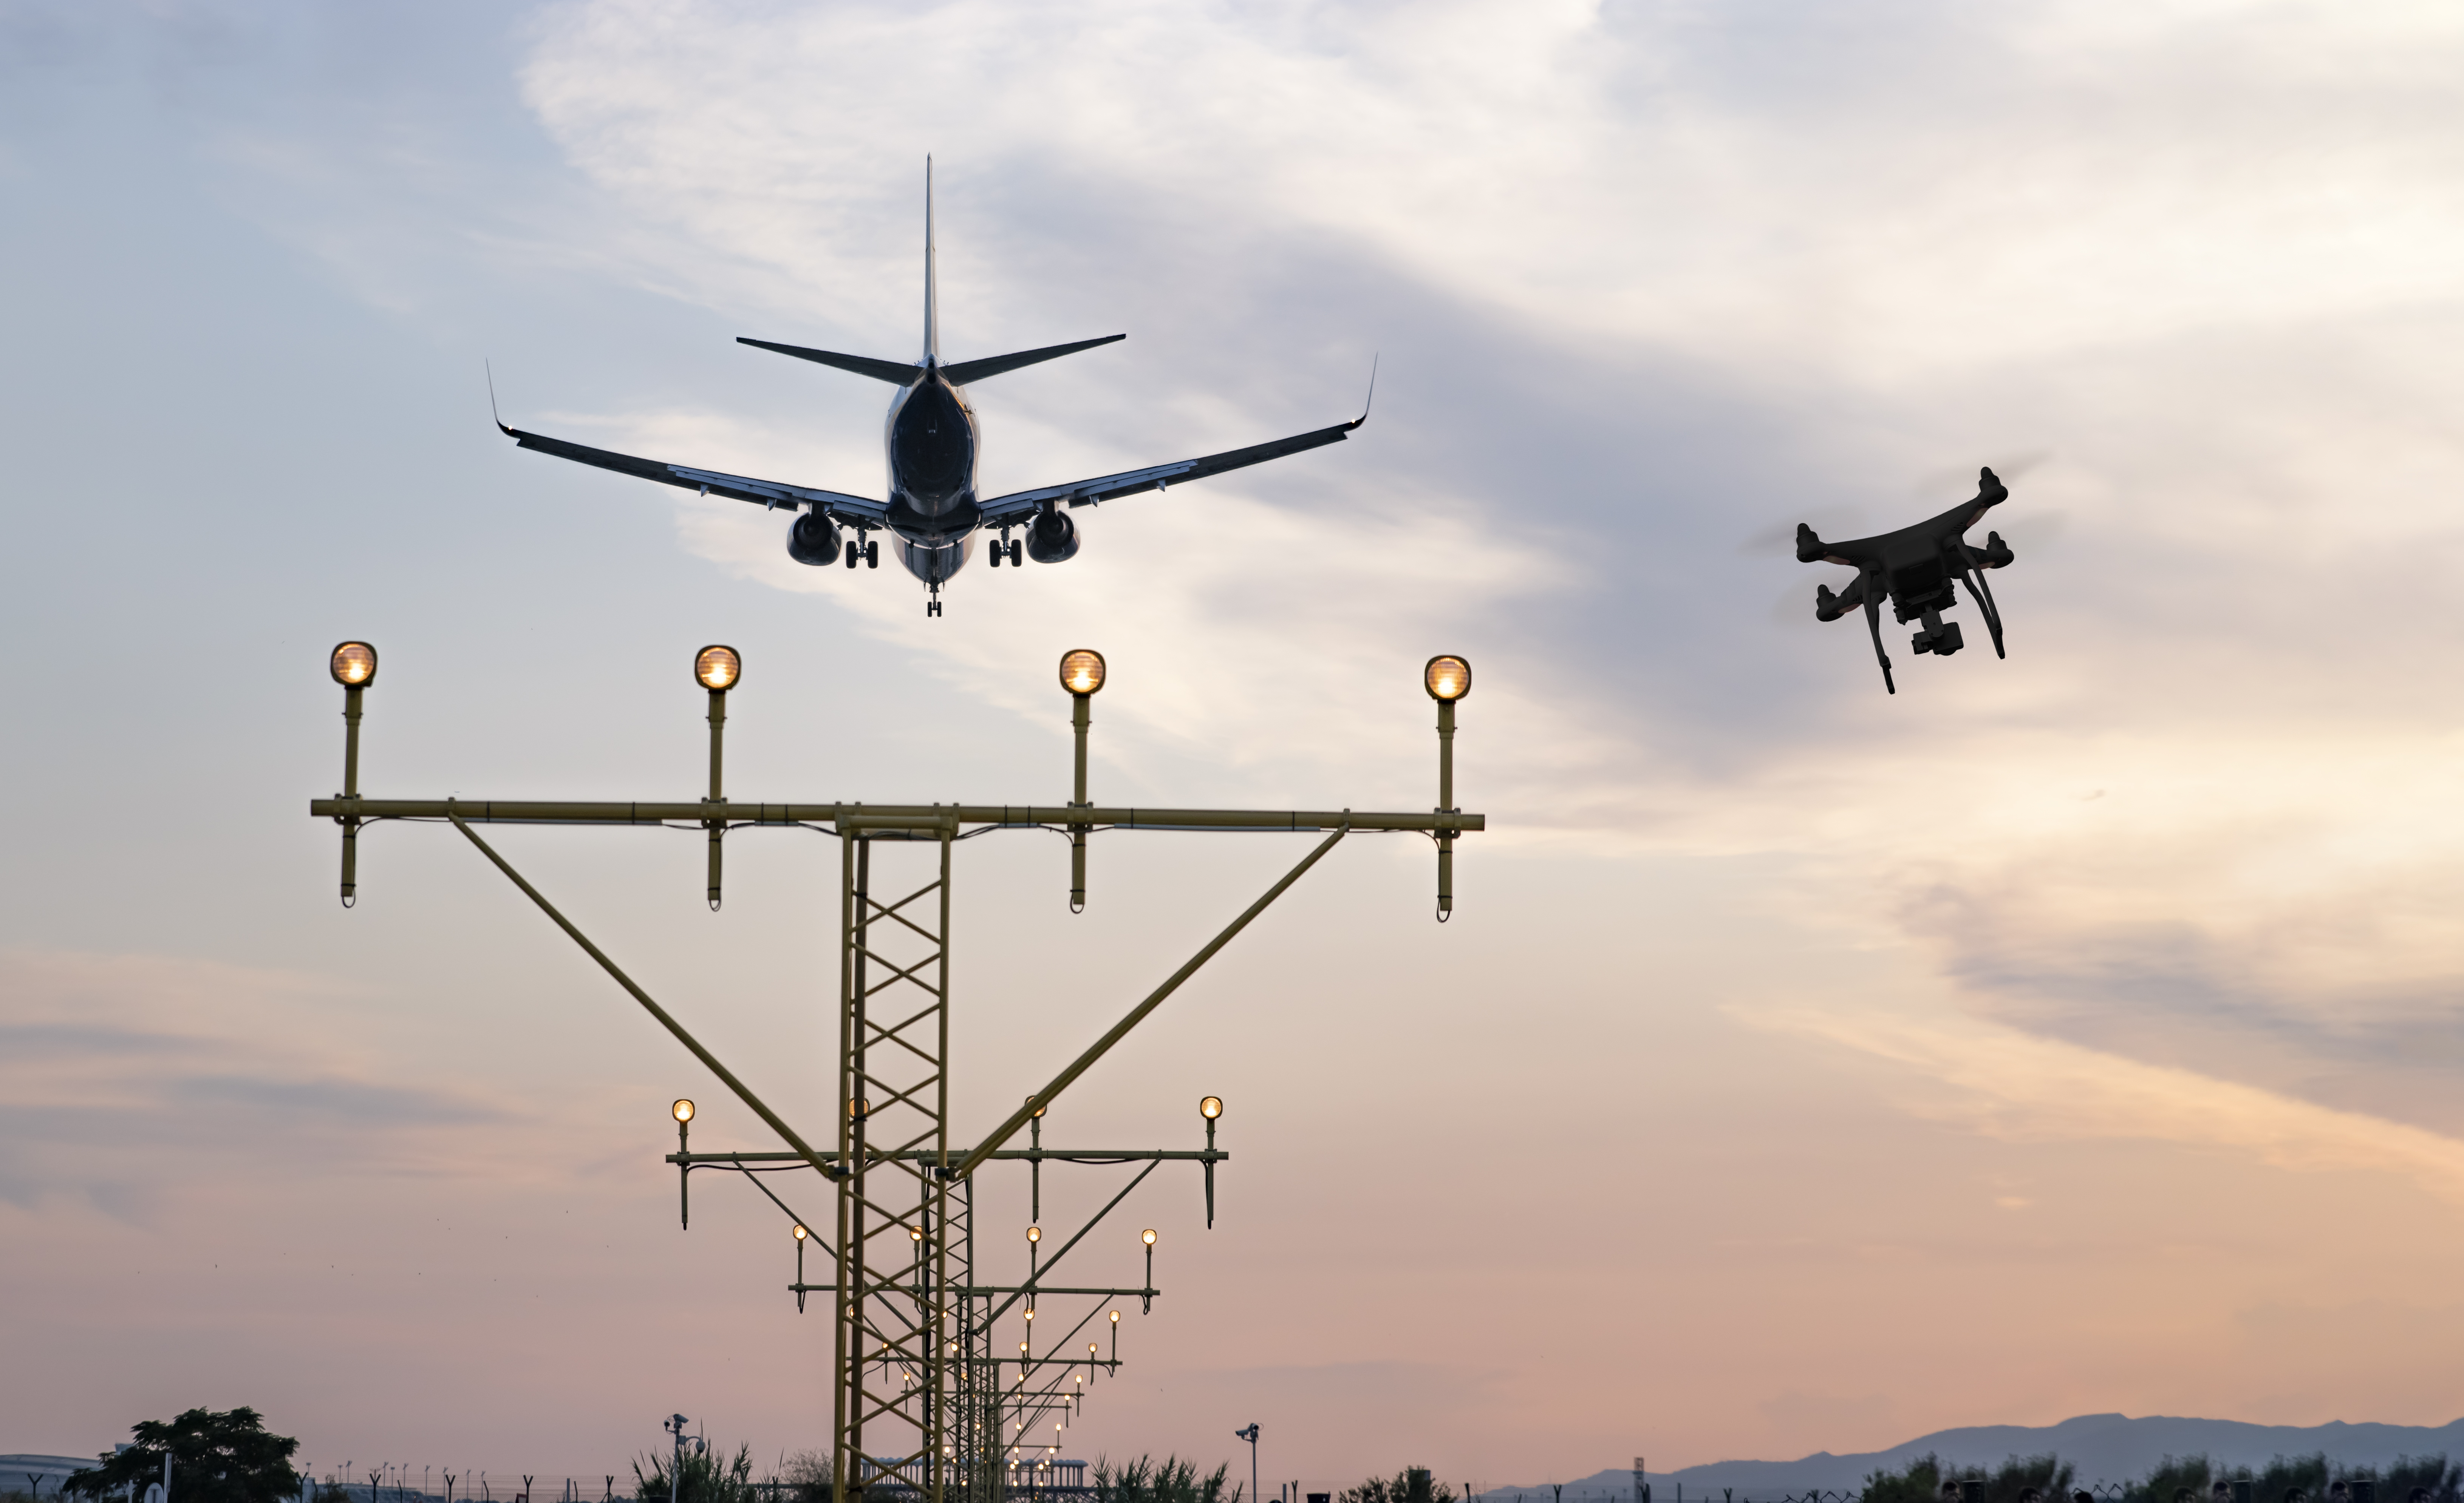
\includegraphics[width=10cm]{imgs/drone_with_plane_landing.jpg}
    \caption{Unauthorized drone near airport.}
\end{figure}




\section{Operational environment}
Great importance is given to the analysis of the context in which detection intends to operate. It is necessary to take into consideration the possible presence of other systems operating in RF and wireless communications like RFID, cellular network, wireless sensors network which can cause serious problems in the detection instruments. It is possible to refer to this type of environment with 'radiowave environment'. It is very important to choose carefully where to position the operational frequencies within it, in order to not cause interference to nearby systems and at the same time to respect the spectrum regulations that vary from region to region. Among all possible detection solutions for drone defense systems investigated by this thesis the primary one is the radar detection solution. In the figure \ref{specrtum} the frequency spectrum of interest is shown.

\begin{figure}[h!]
    \centering
    \includegraphics[width=13cm]{imgs/ElecSpect.jpg}
    \caption{Electromagnetic spectrum.}
    \label{specrtum}
\end{figure}

Considering the dimensions of drones that are in the range of centimeters, the frequencies need to detect this devices belong to the X, Ka, K, Ku bands. This range goes from 8 to 40 GHz and is a direct consequence of relationship between wavelength and frequency: $\lambda = c/f$. In fact, wavelengths of 1 cm - 10 cm correspond to this range of frequencies.
The current cellular bands are all in sub GHz range of spectrum and don't cause interference to our bands while several bands of 5G cellular network are in the range of frequencies considered and can interfere with the detection system. \\ Another important analysis to be carried out on the context is the physical one, named for simplicity "physical environment". It is possible to identify the physical characteristics of the context in which one intends to operate, characterized by the presence of people, obstacles, multipaths and blind areas that for example can cause a false detection or block the radar waveform. Having defined the two main components that make up the environment, let's now see what are the contexts in which we want to investigate the use of radar technology for drone detection. In general, in relation to the level of risk and the size of the area there are different specific needs for radar technologies and different costs. In a situation of high risk and very large area such as in the case of an airport or an oil refinery, it is not necessary to spare expenses and complexity. As a result, complex military-level solutions are accepted. On the other hand, civil situations characterized by a low budget and the presence of people in the vicinity of detection instruments, in some cases characterized also by a limited temporary duration (event), do not allow the use of military-level and/or fixed solutions. Consequently, in situations such as public events, squares full of people, perimeter areas (homes, prisons, stadiums) it is necessary to adopt solutions characterized by a lower complexity, a lower cost and simplicity of use and installation, all attributes contrary to the military field. \\ Figure \ref{context} shows a general grouping of the situations considered, the main discriminating factor among the contexts is the military and civil attribute. Subsequently it is possible to further subdivide the civil scenario into fixed and mobile solutions. The scenario investigated by the thesis concerns the civil context and all its sub-cases. These contexts are in general small and medium-sized areas such as individual homes, squares and perimeter areas like power plants, prisons, etc. It is necessary to pay attention to the radiowave environment, for example in case of a massive presence of people whereas each of them generally owns a smartphone that can operate in 5G bands and can cause problem to detection radar. For what concern the fixed solution in a civilian context it is easier to imagine a low cost fixed radar, while a real challenge is to be able to create a portable and low cost radar solution. An example for the latter case could be a radar used to protect the confidentiality and privacy of a very limited area, such as the case of a boat. 

\begin{figure}[h!]
    \centering
    \includegraphics[width=13cm]{imgs/Contexts groups.png}
    \caption{Context division.}
    \label{context}
\end{figure}

\newpage
\section{Detection technologies \cite{survey}}
Measurements by means of a radar are not the only ones possible to determine the presence of a drone in the surrounding area. During its flight, a drone can emit several types of measurable quantities such as:
\begin{itemize}
     \item Noisy sound,
         
    \item Heat,
        
    \item Radio frequency signals,
\end{itemize}

Consequently, it is possible to determine its presence by taking one or more of these measurements by the relative instruments that are IR/Optic cameras, acoustic sensors and radio frequency scanners. For the pros and cons of each technique an hybrid solution is preferable, in such a way that where a sensor has a gap it is filled by the other sensor. The radar solution is usually the most used due to the benefits of independence, privacy and performance and in many cases it not need other sensors because is the most complete solution. It follows a brief description of acoustic, thermal and radio frequency solutions. \\ Acoustic sensors are generally array of microphones, that are characterized by very low cost and small dimensions. On the other side this solution is strongly influenced by the presence of all background noises that cause a high alarm false rate. Considering also the short range offered, that is of hundreds of meters, the solution in question is not very useful. Example of use of this technique combined with machine learning achieve 83\% of accuracy and combined with k-nearest neighbors algorithm achieve 61\% of accuracy \cite{survey} \cite{robinradar1}. Unfortunately is not possible to retrieve direction of arrival of sound and perform tracking of drones. Thermal detection technologies allow to measure the heat emitted by the drone by means of infrared or optic cameras. In fact drone's components like motors, battery and hardware produce a significant amount of heat. Usually the measured data is compared with the characteristic IR signature of the drones, as happens for the remote sensing performed in satellite images. Each materials and objects have a characteristic reflectance of the light in a specific portion of spectrum that is a kind of signature. It is possible to use a convolutional neural network to process the thermal images to recognize the spectral signature and identify the possible presence of a drone \cite{survey}. This technique returns excellent results at a very low price but in practice the viewing range does not exceed one hundred meters and in public place there is also the problem of privacy if we consider the presence of cameras. Furthermore, this method is strongly influenced by atmospheric conditions. For all these reasons it can only be used together with other technologies such as radar. For example with a combination of radar and IR camera, the minimum radar detection range problem can be solved. Concerning radio frequency analyzers, they are devices capable of picking up micro waves and analyzing their spectrum. They can be exploited for the benefit of drone detection by intercepting messages exchanged between the drone and the controller. In the context of electronic warfare, this practice falls within the group of action called SIGINT or COMINT that stands for Signal Intelligence or Communication Intelligence. The use of these techniques deserves particular attention as commercial drones are often controlled by a remote pilot and the communication protocols between the drone and the controller are widely known. Therefore this knowledge can be fully exploited to recognize the drone model and undertake hijacking techniques. For example, if the message formats used between the controller and the drone are known, it is possible to create false messages and hijack the drone elsewhere without causing it to fall. Take the drone out from defended area without causing its crash, that can be a very dangerous event, is one of the most effective solution. Using this technique, the position of the drone is obtained from the information that it itself sends to the controller, as happens with the well-known air traffic system ADS-B. Therefore this technique is a dependent type solution, because it depend from the information sent by the drone, and for this reason it cannot be used as the only detection solution: if the drone is in autonomous flying mode or if the communication protocol of the messages exchanged with the controller is not known, it is impossible to detect it. Usually considering the extreme simplicity of implementation of these systems and their low cost, they are widely used and are often chosen as a drone detection solution together with a radar technology. With a solution of this type is also possible to localize a drone also if it doesn't communicate the information of location to their controller. For example, by using multiple RF receivers and by applying a type of multilateration technique \cite{survey}. It is important to clarify that also in this case is necessary to know the messaging protocol. Another possible use of RF scanner technique is within a neural network that perform the operation of classification of stolen signals \cite{survey}. So the advantages of a RF scanners are the low cost, the possibility to localize the drone also with multilateration technique and simplicity of implementation. On the other side a reasonable cons is the impossibility to detect drone in autonomous flight mode and that use a unknown protocol of messages. Current manufacturers of anti-drone technologies, to avoid blind spots, implement multiple detection systems with sensor fusion technology. A typical example of radar plus EO/IR sensor camera is shown in figure \ref{EOcamera}. This is one of the most complementary solution for drone detection because is possible to identify a threat seen by the radar at long distance by means of the EO/IR scanner that confirm or refuse the detection from radar. In this way the short range problem of EO/IR scanner is resolved by the radar and the low accuracy or identification problem of radar is resolved with the EO/IR scanner. So, also in the most part of commercial implementations the radar is seen as the main technology to detect  a drone and other sensors can be used together to achieve accuracy improvement.
\begin{figure}[h!]
    \centering
    \includegraphics[width=9cm]{imgs/radar + eo camera.jpg}
    \caption{Radar + EO scanner configuration.}
    \label{EOcamera}
\end{figure}

Another detection configuration, that does not involve the use of radar, could be the multiple RF sensors, which by combining the intercepted information between them is possible to locate and to track a target drone. An example is shown in the next figure.

\begin{figure}[h!]
    \centering
    \includegraphics[width=6cm]{imgs/RF scanner triangulation.png}
    \caption{RF scanners triangulation \cite{survey}.}
\end{figure}
\newpage

Even if the drones does not exchange information about its location, it's possible to locate it by measuring the time of arrival of messages at each RF receiver. But it is necessary that the intercepted radio frequency messages are with certainty associated with a drone present in the area. Obviously with this configuration it is not possible to identify a drone that does not exchange messages of any kind or whose message exchange method is unknown. Another hybrid combination is possible by means of radar plus acoustic sensors, that is another accuracy improvement for the radar solution. In table \ref{tab:Hybrid_solutions} are shown the hybrid solution proposed by the vendors and their range performance.
\\

\begin{table}[!h]
\begin{tabular}{|
>{\columncolor[HTML]{FFFFFF}}l |
>{\columncolor[HTML]{FFFFFF}}l |
>{\columncolor[HTML]{FFFFFF}}l |}
\hline
{\color[HTML]{000000} \textbf{Vendor, Model}}    & {\color[HTML]{000000} \textbf{Combined techniques}}           & {\color[HTML]{000000} \textbf{Range}} \\ \hline
{\color[HTML]{000000} ELTA, Droneguard}          & {\color[HTML]{000000} Radar + RF scanner + Camera}            & {\color[HTML]{000000} 4.5 km}         \\ \hline
{\color[HTML]{000000} Aaronia, AARTOS DDS}       & {\color[HTML]{000000} Radar + Camera}                         & {\color[HTML]{000000} 5 km}           \\ \hline
{\color[HTML]{000000} APS, Ctrl+sky}             & {\color[HTML]{000000} Radar + RF scanner + Camera + Acoustic} & {\color[HTML]{000000} 3 km}           \\ \hline
{\color[HTML]{000000} Cerbari}                   & {\color[HTML]{000000} RF scanner  + camera}                   & {\color[HTML]{000000} 3 km}           \\ \hline
{\color[HTML]{000000} Rodhe e Schwartz, Adronis} & {\color[HTML]{000000} RF scanner}                             & {\color[HTML]{000000} 3 km}           \\ \hline
{\color[HTML]{000000} Droneshield, Sentinel}     & {\color[HTML]{000000} Radar + RF scanner + Camera + Acoustic} & {\color[HTML]{000000} 3.5 km}         \\ \hline
\end{tabular}
\caption{Hybrid solutions \cite{survey}.}
\label{tab:Hybrid_solutions}
\end{table}

%\begin{figure}[h!]
 %   \centering
 %   \includegraphics[width=16cm]{imgs/Tabella hybrid.png}
 %   \caption{Hybrid solutions}
%\end{figure}





\clearpage

\section{Complete anti drone system}
A complete anti drone system must be able to perform all the actions necessary to block a drone, all the phases that the system must do are:
\begin{itemize}
     \item Detection phase;
         
    \item Identification phase;
        
    \item Neutralization phase.
\end{itemize}
It is important to clarify the different phases that an anti-drone system must carry out. In particular, considering the detection process, which we are interested in, it must necessarily also include a primary identification phase. This task is only to verify that detected object is a drone, while the next identification phase is necessary to distinguish between friend or foe drone and to evaluate the level of risk associated to it. For example, a drone can be easily confused with a bird or any other flying object. Consider that many hybrid solutions include a low-cost radar, it does not also implement the functionality to distinguish them which is instead delegated to another component as we have seen in the case of a radar plus EO/IR sensor configuration. On the other hand, there are more expensive radars that are able also to carry out the primary identification phase and therefore they can distinguish a drone from an object of the same size. For example, this operation can be done through spectral analysis, identifying the presence of rotating blades \cite{robinradar2}. It's important to to underline that this primary identification phase belongs to the detection phase and it is different from the next one identification which constitutes a completely separate phase. This is the task of understanding if the detected drone is a threat or not. In practice the result of this phase is to respond to the question: 'Is necessary to neutralize the detected drone?'. In a first experimental implementation based only on detection phase, we can simply assume that the area to be monitored does not admit the presence of any type of drone, friend or foe. In a more advanced implementation, however, it is possible to consider the presence of friendly drones and enemy drones and therefore we need to find a way to distinguish them. This task can have different solutions, for example a friend or foe style RFID technique can be used. In this case distance and speed are challenges since velocity can be very high and range must be very short. Another solution can be to track and then analyze the path of the drone by means of machine learning and neural networks. In this way is also possible to predict the drone's action and recognize a friend drone. This type of technique is the most suitable for a radar system because, unlike the RFID solution, it is also of independent type and don't need external information in addition to those provided by the radar. Another possible solution, dependent like RFID technique, is to adapt the ADS-B or FLARM system to drones \cite{survey}. The main difficult is the dimension of ADS-B module, but uAvionix propose the Ping2020 that is a family drone-ADS-B. The main limitation in this case is the price  that is very high. FLARM is less expensive solution primarily designed for light weight UAS (Unmanned Aerial Veichle) but it's encryption protocol add extra processing time and it is proprietary. \\
Once the drone is detected and confirmed as a threat can be very useful to estimate the level of risk associated to it. To do this is possible to implement a math model that associate a numerical risk value to the threat. For example a math equation like this can be used: 
$R=\left(R_{\text {object }}+R_{\text {path }}\right)^{R_{\text {time }}}$
\cite{survey}.

In general is necessary to classify the different areas in the supervised zone in relation to their risk, as is done with the ICAO area classification. Then the first value of risk $R_{\text{object }}$ come from the mass and velocity of drone that express its kinetic energy. This information come from the detection phase where in relation to the drone dimension a mass can be deduced, while velocity is properly measured by means of the Doppler frequency. Then, at this value is added the risk $R_{\text{path}}$ related to the actual position of drone, directly proportional to the area classification risk. Also proportional to the direction of drone's path and distance to the other areas by means of weighted sum. A picture where the drone flight direction and different areas with different risk is shown in figure \ref{risk}. Finally $R_{\text{time }}$ is related to the response time of neutralizing system that are described below.

\begin{figure}[h!]
    \centering
    \includegraphics[width=12cm]{imgs/Risk model.png}
    \caption{Different risk area related to drone path.}
    \label{risk}
\end{figure}

%soluzioni di neutralizzazione
Once the threat has been identified and its level of danger assessed, action must be taken. So the last step of an anti drone system is the neutralization. In general is possible to distinguish two type of neutralization technique:
\begin{itemize}
     \item Destructive techniques: in which the use of weapons is accepted that cause the fall down and consequent destruction of the drone. So this is a type of military solution;
         
    \item Non destructive techniques: where the use of military weapons is not admitted and is not possible to cause the fall down of the drone, so it is the most addicted solution in a civilian environment where the people are close to the target drone;

\end{itemize}

One of the most desirable non destructive technique is the drone hijacking. This neutralization solution is the safer technique, in fact the unauthorized drone is moved out the supervised area in a safe way. In practice a defender operator take the control of unauthorized drone in two stage. During the first stage he cause the disconnection between the original controller and the drone, breaking the pairing between them. Then during the second phase the defender operator execute the pairing with the drone and so became the new controller \cite{survey}. It's important to note that this neutralization solution is possible only if the attachment procedure with the drone is fully known and if the drone is not in an autonomous flight mode. This technique includes hacking and spoofing practices. In the next picture is shown a representative scheme of this technique.

\begin{figure}[h!]
    \centering
    \includegraphics[width=10cm]{imgs/Drone hijacking.png}
    \caption{Hijacking technique.}
\end{figure}

Another possible solution of neutralization is the spoofing technique. Considering that most of the commercial drone have a GPS module and rely heavily on the information received from it, is possible to send them a fake GPS position in order to confuse them. This technique is possible also when the drone is not controlled by a remote operator and is in autonomous flight mode.
Another possibility is the geofencing technique that is already implemented in almost all commercial drones. In practice, relevant areas such as an airport are saved into a database that is a collection of all restricted area for drones. Then many commercial drones are also equipped with an autolanding module that prevents the invasion of restricted area by accessing the database of restriction and controlling them. Obviously by modifying the commercial drone and eliminating this module is very simple to evade this check. These are the most used techniques for the non destructive set in which we are interested. Then for completeness also few destructive  technique are listed below. Killer drones are called the practice of attack or damage of enemy drones by means of friend drone. Drone capture is instead the practice of capturing the unauthorized drone by means of net in a terrestrial or aerial way. Also the jamming can be considered as a destructive technique because it can cause the drone to fall. Is possible to distinguish different kind of jamming in relation to the direction, the position and the bandwidth of jammer. A very useful approach can be the GPS jamming because the GPS protocol is fully known instead the messaging protocol of the drone can be unknown. As mentioned above, however, jamming solutions are unusable in the civil field not only for the possibility of causing a fall but also for the regulation of the spectrum and interference to other telecommunication systems. While the other mentioned destructive techniques are not usable in a crowded context for the safety of people.
Another important consideration are done for better design a complete drone defense system. Considering the rapid evolution of drone technology, and the different instrument of detection used is necessary to design a modular system, in this way, each component can be updated and will help keep the system up-to-date.
